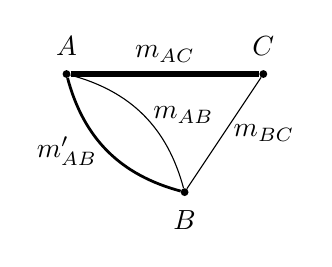
\begin{tikzpicture}[node distance=10pt]
\tikzstyle{blackdot} = [circle,fill, scale=0.3];

\node [blackdot] (v1) at (-1.5,1) {};
\node [blackdot] (v3) at (1,1) {};
\node [blackdot] (v2) at (0,-0.5) {};
\node[above of=v1] {$A$};
\node[above of=v3] {$C$};
\node[below of=v2] {$B$};
\draw[bend left]  (v1) edge node[right] {$m_{AB}$} (v2);
\draw[bend right,line width=1pt]  (v1) edge node[left] {$m_{AB}^\prime$} (v2);
\draw  (v2) edge node[right] {$m_{BC}$} (v3);
\draw[line width=2pt]  (v1) edge node[above] {$m_{AC}$} (v3);

\end{tikzpicture}
